\chapter{Project Methods}
\label{chap:projectsteps}


\section{Introduction of Note Sets as a new note data container}

We will introduce Note Sets as a new data container for referencing and persisting sets of note data. While these Note Sets will be exported to files, they do not constitute a file format in the narrower sense, but rather a new paradigm as how to think of collection of notes: No longer as notes that were recorded in the same transaction and thus in the same binary file (in earlier times this was the only way one could think of collections of notes), but as a collection of IDs.

The note set data container will have the following advantages:
\begin{itemize}
\item Compactness: Note Sets will be minimalist in the sense that notes are references by ID only. There is no additional information like annotation stored in the note set format.
\item Independency of file locations: With the introduction of MFX the actual location of a file in the pool becomes redundant. Therefore, the note set does not store any file paths.
\item Equivalence with respect to annotation: Unlike the Notelist format, Note Sets will no longer have an individual annotation per note. Rather, they have at most one annotation per note set, which is to be persisted in the note set's filename. Thus, note sets are considered equivalent with respect to annotation
\end{itemize}
Meanwhile, the new data container must at least satisfy the following requirements:
\begin{itemize}
\item Convertability to and from the existing Notelist format. The Notelist format has been established as the standard way of storing data sets in Currency Adaptation. Even if one were to pursue the goal of replacing the Notelist format by the Noteset format, convertability would be needed at least for a period of transition. The reasons for that are that a) Noteset import is supported by MCM however in a yet limited way. b) the Python MCM wrapper library mcmp, which is used to load notes and run algorithms from outside MCM, does currently not support the loading of Notesets.
 \item Differentiability. Since they are so minimalist, Note Sets are more ideal than previous formats for quick comparison. We need a way to compare and find the difference between Note Sets reliably and efficiently.
\end{itemize}

The Note Set data container will be introduced in a small python library providing the abovementioned functionality. This library is then deployed as a python package and can be used in the python toolchain, including MDS and MFX, as well as in Jupyter notebooks. In a later step it remains to analyze the feasibility of introducing this data container in the .NET toolchain as well.

\section{NoteSet Generation}
Using different methods and for a set of exemplary currencies a first version of NoteSets are generated from the Data Pool, In the course of this existing client software of MDS and MFX are extended to allow for more complex queries.\par
In a first phase Jupyter Notebooks will be used to generate the NoteSets. Different methods and their results, i.e. the resulting NoteSets, will be compared and presented to the Currency Adaptation Team. Once the NoteSet generation process has been refined on a technical level, it remains to decide how to include it in the adaptation specialist's workflow.\par
The NoteSet generation workflow in this development phase can be described as follows: 
\begin{enumerate}
\item Crawl MFX for a chosen currency to obtain all file paths of .NIF files for that currency
\item With a list of all FileIDs and corresponding filepaths, use a labeling method to label all the notes in alle the files
\item Based on the obtained labeling, split the set of all Notes into labelled NoteSets (within a NoteSet, all elements have the same label)
\end{enumerate}
It remains thus to choose a labeling method. The following methods will be used and compared
\begin{enumerate}
\item For each note in the set of all notes, query MDS to obtain the recognition and classification done by the reader for this note. We use the banknote reader (and the CDF which was loaded at the time of recording) as the labeller.
\item Load all the notes from the set of all notes into MCM and use algorithm(s) from the algorithmic framework of MCM to determine properties of each note based on which the notes can be labelled. We use MCM as the labeller. To do this in an automated way, a Python wrapper for MCM has to be used, which unfortunately only allows restricted use of MCM.
\item Use an algorithm external to MCM as a kind of plug-in to process and label the notes. This is the most experimental method, but maybe also the most interesting one. It has the advantage that we are free of MCMs monolithic architecture in our labeling process, but also the challenge that the MCM algorithmic framework is highly developed and refined and can hardly be bested by an external classifier.
\end{enumerate}
\par The following figure illustrates the three methods

\begin{figure}[!htb]
\minipage{0.32\textwidth}
  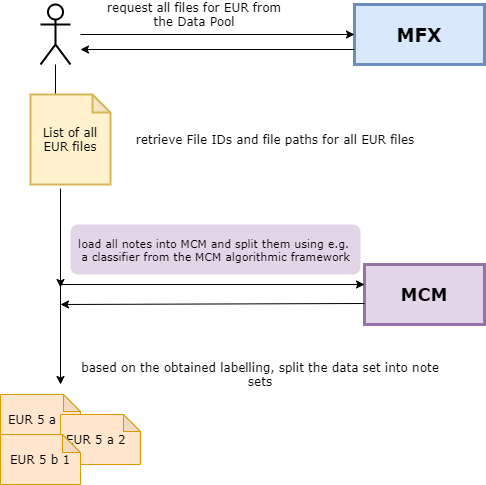
\includegraphics[width=\linewidth]{images/label_mcm_approach.png}
  \caption{A really Awesome Image}\label{fig:awesome_image1}
\endminipage\hfill
\minipage{0.32\textwidth}
  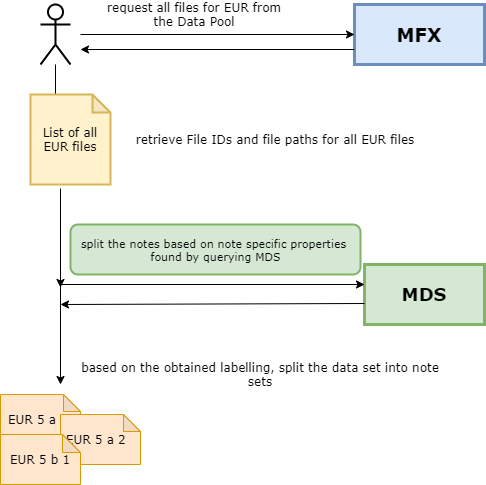
\includegraphics[width=\linewidth]{images/label_mds_approach.png}
  \caption{A really Awesome Image}\label{fig:awesome_image2}
\endminipage\hfill
\minipage{0.32\textwidth}%
  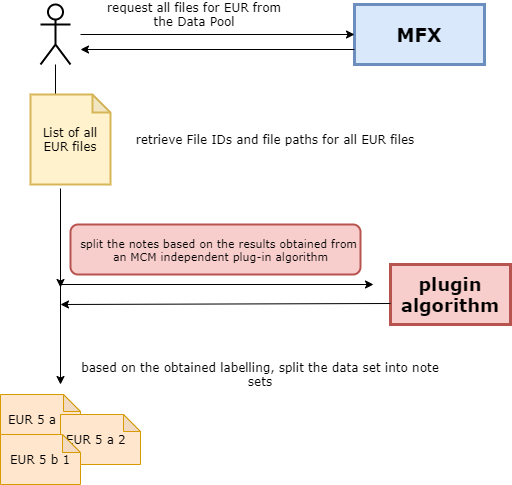
\includegraphics[width=\linewidth]{images/label_plugin_approach.png}
  \caption{A really Awesome Image}\label{fig:awesome_image3}
\endminipage
\end{figure}

\section{Feasibility of NoteSet replacing Notelist in the entire Toolchain}
In a next step an analysis is done of what it would mean to replace the standard Note Data Container Notelist by the newly introduced NoteSet. Especially, how complex costly it would be to refactor the main adaptation tool MCM to work with NoteSets. This is important because MCM will always set the standard of the currency adaptation workflow and if NoteSets are to be the standard data container, MCM needs to be able to handle them in an efficient and user-friendly way.